\documentclass[12pt,a4paper]{article}

\usepackage{amsfonts,amssymb,amsmath,amsthm}
\usepackage{stmaryrd} %for special brackets
\usepackage{lipsum}
\usepackage{graphicx}
\graphicspath{img}
\usepackage[hidelinks]{hyperref}
\usepackage{array}
\usepackage{bm} %for bold in math equations
\usepackage{float} %to force the position of some figures
\usepackage{biblatex}
\usepackage{geometry}
\usepackage{todonotes}
\usepackage{multirow}

\addbibresource{_report.bib}
\geometry{left=2.54cm,right=2.54cm}


\title{Internship Report}
\author{Lucas SALAND}
\date{\today}

\begin{document}
\maketitle
\newpage
\tableofcontents
\newpage

\section*{Introduction}
This M1 internship was carried out at CRIStAL in the SIGMA team under the supervision of Patrick Bas. The internship lasted for three months during which we worked on a challenge from the AID on the detection of images generated by AI.\\
CRIStAL is a laboratory which research focus on computer science, signal and automatic control. It is under the supervision of the University of Lille, CNRS and Centrale Lille. The laboratory is divided in 34 research teams grouped in 9 Thematic Groups. SIGMA team is part of DatInG : Data Intelligence Group. SIGMA is a team of 15 permanent staff which focuses on machine learning, statistics and signal processing. Some of the research topics are Monte-Carlo methods, signal processing with tensorial approaches and information security.
\todo[inline]{develop on the team environment (saw a phd defense, sigma day)}

The Agence de l'innovation et de défense (AID) launched a challenge on detecting modified or generated images. This challenge aimed at detecting three types of images :
\begin{itemize}
    \item fully AI-generated images;
    \item images partially modified by AI;
    \item images partially modified with more usual image processing tools such as photoshop.
\end{itemize}
This challenge was divided in two tasks : A and B. Task A focused on images fully generated by AI. AId first provided a sample of images to give an idea of what would be the testing data would be. Images provided were compressed with JPEG. Our team identified 3 quality factors for compression: 40, 65 and 90. AID then provided 10000 images on the last day of the challenge. The goal was to identify which images were real and which one were generated. On top of this, we could provide which generator was used to generate images. Task A could be treated as binary classification problem with the two classes being real and generated images. It could also be treated as a multi-class classification problem where the classes would be the real images and all the generator used. The main difficulty was that the generators used were kept secret until the last day of the challenge.\\
Task B focused on the detection of partially modified images. The objectives were :
\begin{itemize}
    \item detecting real images and modified images;
    \item identifying the tool used for modification;
    \item localisation of modification on images.
\end{itemize}

I worked on the challenge in a team with 3 other interns and 5 permanent staff from SIGMA. During the internship, I worked on task A.


\section{AI-generated images detection}
\subsection{AI image generation}
We should now go over an overview of image generation with AI. In recent years, the quality of images generated with AI models skyrocketed. These models appear as promising new tools for art generation and data augmentation for machine learning. In 2014, Generative Adversarial Networks were introduced by Ian J. Goodfellow and his colleagues in \autocite*{goodfellowGenerativeAdversarialNetworks2014}. A GAN is composed of two main components : a generator and a discriminator. The generator take random vector as input and tries to generate images that are indistinguishable from real images. It tries to fool the discriminator. On the other hand, the discriminator's goal is to differentiate between real data from the training set and fake data produced by the generator.
\begin{figure}[H]
    \centering
    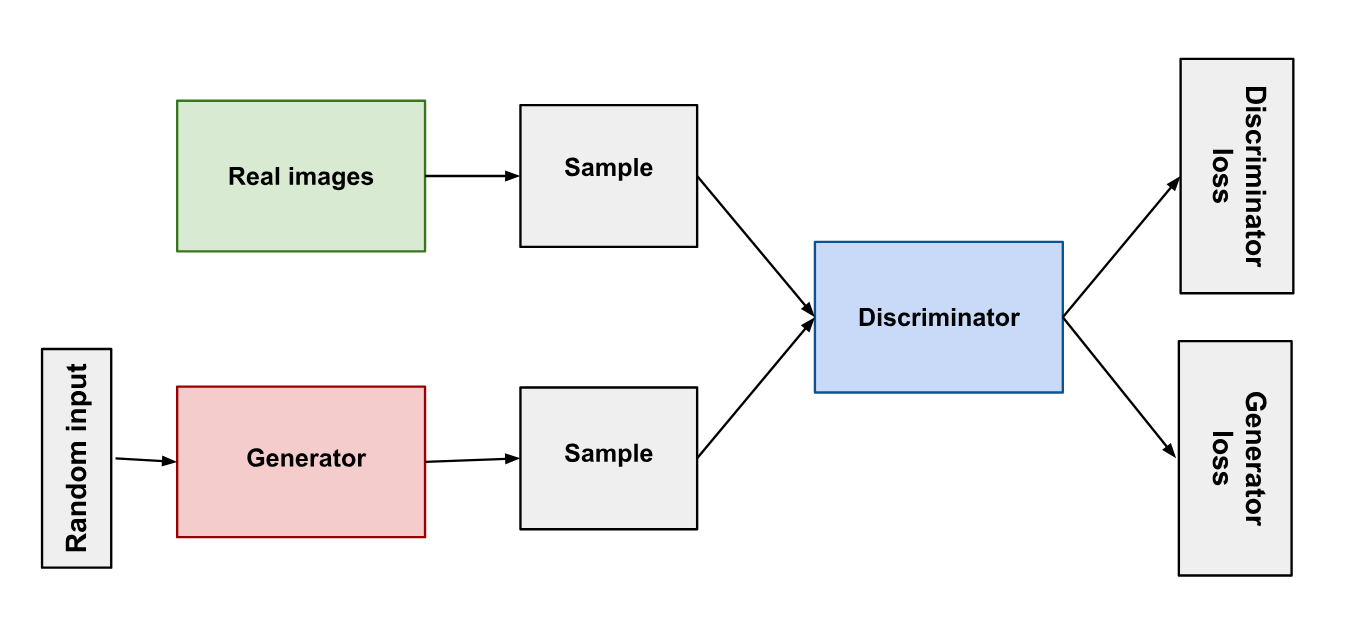
\includegraphics[width=\textwidth]{img/GAN.png}
    \caption{GAN architecture}
\end{figure}

Diffusion models use a different approach to generate images.
\todo[inline]{More on diffusion model}


As improvements happen at an impressive rate in the field of generative models, concerns about security issues rose as well. These tools could be used to manipulate information and combined with social media they would be weapon of massive disinformation. As generative model keep improving, we need to develop new tools to detect generated images. But what should we look for in generated images in order to differentiate them from real images? Many approaches were explored in recent years. Let's go over some of them as they are presented in \autocite*{tariangSyntheticImageVerification2024}.

\subsection{Detection based on high-level artifacts}
These methods detect generated images using a similar approach as humans when they differentiate real and generated images. These approaches look at errors such as incorrect perspectives, incoherence in lighting and shadows or asymmetries in faces.

\subsection{Detection based on low-level artifacts}
AI-generated images contain artifacts in the Fourier domain of the model used to generate them. Detecting these traces is a way to detect whether an image is AI-generated. Many generation models contain an upsampling operation in their generation pipeline. An alternative approach to exploit high-frequency artifacts is to look at the noise residuals by removing the scene content. Nonetheless, these approaches are weak to post processing of images. If for instance, jpeg compression is applied, low-level information can be lost making it impossible to correctly classify an image.
\begin{figure}[H]
    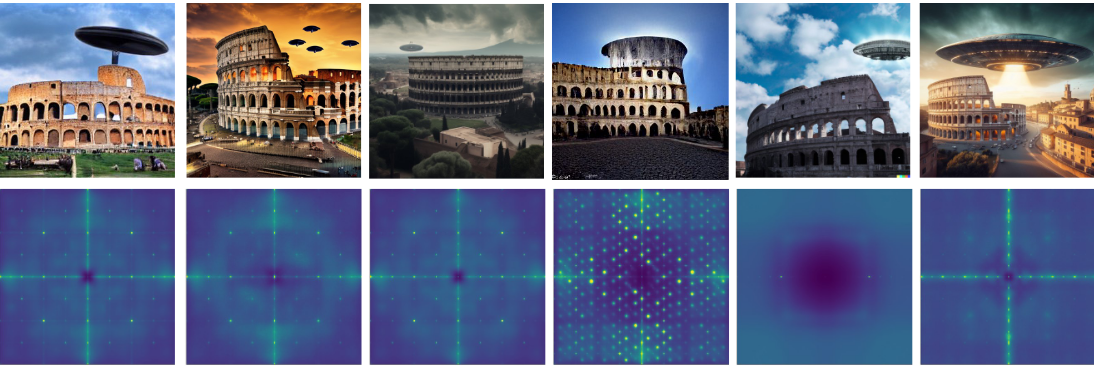
\includegraphics[width=\textwidth]{img/peaks.png}
    \caption{Figure and caption extracted from \autocite*{tariangSyntheticImageVerification2024}. Top: examples of synthetic images, generated using (from left to right) Latent Diffusion, Stable Diffusion, Midjourney v5, DALL·E Mini, DALL·E 2, DALL·E 3. The prompt used for their generation is the following: a photo of the Rome Colosseum with a UFO over it, detailed, 8k. Bottom: Average Power Spectra of the artificial fingerprints for each of such model. Forensic artifacts are clearly visible as spectral peaks in the Fourier domain, stronger or weaker based on the specific model. We can observe that the first three images share very similar artifacts while the fingerprints of the three releases of DALL-E differ greatly from one another, testifying to very different generative architectures.}
\end{figure}

\subsection{Data-driven approaches}
Early method for synthetic image detection were based on CNN architecture with a lot of data. Trying to learn useful features that could help differentiating real and generated images. These first approaches worked well when training and testing data were very similar but had poor generalization capability. To address this robustness issue, researchers used deep CNN architectures combined with augmentation at training time. Augmentations included compressed and blurred images. The diversity of the data used for training also plays a crucial role in a detector's ability to generalize. More recent works delved into architectures different from CNN. In \autocite*{cozzolinoRaisingBarAIgenerated2024}, authors showcased the good performances of CLIP-ViT\footnote{ViT: Vision Transformer} for this type of classification. Within my team, I worked on a semantic approach using CLIP and \autocite*{cozzolinoRaisingBarAIgenerated2024} as a starting point.\\
CLIP (Contrastive Language-Image Pretraining) is a neural networked introduced by OpenAI in \autocite*{radfordLearningTransferableVisual2021}. This network was trained on a massive amount of (text,image) pairs and can then be used with no modification for zero-shot classification. This network training is called contrastive learning. The goal of contrastive learning, as it is stated in \autocite*{tianContrastiveMultiviewCoding2020}, is to learn an embedding that contrasts samples from two distributions. In the case of CLIP, we consider the training dataset to be the following : $\{t_i,\ img_i\}_{i=1}^N$ where $t_i$ is the text associated to the image $img_i$. Each pair contains a textual representation and a visual representation of the same object. We can consider that we thus have a distribution of texts and a distribution of images, which are the marginals, and we have the joint distribution which is the one of the pairs of texts and images. Contrastive learning will separate samles of the joint from sample of the product of marginals. In practice, the model learns to maximize in a latent space the cosine similarity between congruent pairs (e.g.\{"cat", image of a cat\}) and minimize cosine similarity between incongruent pairs (e.g. \{"dog", image of cat\}). As we work in a latent space, it implies that we have encoders to perform the embedding. In the case of CLIP-ViT, transformer-based architectures are used for both the text encoder and the image encoder. Many pretrained versions of CLIP are available online. In our case we used the model proposed by LAION: CLIP ViT-L-14, an open source implementation of CLIP trained on DataComp-1B, a dataset of 1.28B pairs of (text, image) pairs.
\begin{figure}[H]
    \includegraphics*[width=\textwidth]{img/CLIP.png}
    \caption{Figure from \autocite*{radfordLearningTransferableVisual2021}. Images and text are embedded in a latent space, the cosine similarity is then computed on pairs of texts and images.}
\end{figure}

\section{Contributions and associated results}
The first step of building our CLIP detector was to start with something simple. Three ingredients were needed:
\begin{enumerate}
    \item A CLIP model
    \item A dataset with real and generated images
    \item A support vector machine to perform the classification
\end{enumerate}

\subsection{Implementation of a first pipeline toward a CLIP detector}
The CLIP model was obtained through the open-clip library. The weights are loaded from HuggingFace. As a first dataset, we chose ELSA\_D3. This dataset contains 2.31 million quintuples of images. Each quintuples contains one real image and four images generated from a description of the real image with four models of stable diffusion. The dataset being too big for our need and for the available storage space, we only used a small subpart of it. To build our first dataset, we used the datasets library from HuggingFace. We streamed the ELSA\_D3 dataset from HuggingFace and downloaded 10 000 samples from it. At first, we only downloaded pairs of one real image and one generated image from one generator only. Later, we took pairs of one real image and one generated image from a randomly selected generator among the four availables in ELSA\_D3. ELSA\_D3 only contains URLs to the images to download and not the images themselves. Thus, many URLs were dead links. So the code used to download the images had to take into account the possible errors that could occur such as invalid URLs or connection timeout. 

\begin{figure}[H]
    \includegraphics*[width=\textwidth]{img/ELSA.png}
    \caption{An example from ELSA\_D3}
\end{figure}

At first the dataset we created contained the images themselves and every time we wanted to train the SVM\footnote{Support Vector Machine} we had to apply the preprocessing to the images before feeding them to the CLIP model to obtain their embedding. This process being time consuming, we decided to store the features in the datasets instead of the images which lead to significant time savings. The whole process to obtain a classifier was the following :
\begin{itemize}
    \item Load the train/test splits of images
    \item Appply CLIP's preprocessing to all images
    \item Feed the images to CLIP's image encoder
    \item Train an SVM on the CLIP features of the images
    \item Test the SVM
\end{itemize}

\subsection{Impact of JPEG compression}
At first, the SVM was trained on a mix of jpeg and png images. As the sample of images given for the challenge were all jpeg, we decided to convert all images to jpeg. We created datasets for three different quality factors: 40, 65 and 90. These quality factors were chosen based on the early investigations performed on the sample images provided by AID. JPEG compression leads to loss information on the images. Thus we expect that a detector trained on images with high quality factors might perform poorly on  images that are compressed with a low quality factor. 
\begin{figure}[H]
    \includegraphics*[width=\textwidth]{img/jpeg.png}
    \vspace*{-.8cm}
    \caption{Visual impact of JPEG compression}
\end{figure}

To observe the impact of the quality factor on the performances of the detector, we created three datasets, one per quality factor. These datasets are then divided in train and test splits. For each quality factor, we trained the model on the corresponding dataset and tested it ont the 3 test sets. Each dataset contains 10000 elements. We obtain the following results:
\begin{table}[H]
    \centering
    \begin{tabular}{|c|c|c|c|c|}
    \hline
    & \multicolumn{4}{c|}{Test} \\
    \cline{2-5}
     & quality & 40 & 65 & 90 \\
    \hline
    \multirow{3}{*}{Train} & 40 & 0.9813 & 0.9730 & 0.9797 \\
     \cline{2-5}
     & 65 & 0.9450 & 0.9825 & 0.9830 \\
     \cline{2-5}
     & 90 & 0.7744 & 0.8581 & 0.9925 \\
    \hline
    \end{tabular}
    \caption{Accuracy of binary classification for pairs of train/test different quality factors}
    \label{table:jpeg}
\end{table}

As we can obeserve on \autoref*{table:jpeg}, the quality at which images where compressed has an important impact on the average acuracy for binary classification. Looking at the row for quality 40, the accuracy only decrease by a small amount when the testing is perform on images with higher quality factor whereas the acuracy decrease by a significative amount when the data used for training as a high quality factor of 90 and is tested on images with lower quality factor. This result highlight the necessity to add jpeg compression at low quality factor in the training data to obtain better performances.

\subsection{Adding diversity to the data}
We saw in the previous section that our detector as good accuracy when trained on a small quality factor ans tested on other dataset with equal or higher quality factors. But these tests do not give information about the generalization capabilities of our detector. We need to experiment and observe how the SVM classifier performed on images generated by models that are not in the training data. To do so, we used the Synthbuster dataset that was introduced in \autocite{bammeySynthbusterDetectionDiffusion2024}. This datasets contained images generated by 9 different models:
\begin{itemize}
    \item DALL-E 2
    \item DALL-E 3
    \item Adobe Firefly
    \item Midjourney v5
    \item Stable Diffusion 1.3
    \item Stable Diffusion 1.4
    \item Stable Diffusion 2
    \item Stable Diffusion XL
    \item Glide
\end{itemize}

For each generator, 1000 images were generated. This dataset contained only generated images. For testing, we need both real and generated images. Thus we added 9000 images from ELSA\_D3 that were not used in the previous datasets we created.
After training on 10 000 images from ELSA\_D3 with quality factor 40 and testing on synthbuster we obtained an accuracy of 0.64. Our detector was not generalizing well. Two ideas were proposed to improve detector's performances:
\begin{itemize}
    \item Train a multi-class classifier and use it as a binary classifier
    \item Add more diversity in the training data in terms of generators.
\end{itemize}

Implementing the multi-class classifier was simple for the SVM as we just replaced binary labels with class labels and replaced the LinearSVC from sklearn with OneVsOneClassifier. We then trained and tested on Synthbuster and plotted the confusion matrix to see if our classifier could differentiate the images from different generators.

\begin{figure}[H]
    \includegraphics*[width=\textwidth]{img/confusion.png}
    \caption{Confusion matrix for a SVM multiclass-classifier trained and tested on synthbuster.}
\end{figure}

The SVM is able to differentiate pretty well generators on which it has been trained on. It made some mistakes between two versions of stable diffusion but this might be because architectures of both models are similar. This result was a first look at multiclass classification performances but test on out-of-distribution data would be required to see the real performances of our detector.

\subsection{Neural network and bigger datasets}
Up until synthbuster, I was gathering dataset by myself over internet. Then, the team decided to share datasets to be more efficient. Therefore, new datasets were added under a common folder on epeautre, the remote machine on which our code was running and our data was stored. The AID dataset was created. This dataset contained 17 generators with 2000 images per generator and 165000 real images from Flickr. In my case I only took a 1000 images per generators and 17000 real images.\\

Besides the AID dataset we used another dateset that we named AID\_TEST which was used to test the model we trained on AID. This dataset contained 32 generators with 1500 images generated for each of them. In addition to that, the dataset contained 40 000 real images. Training and testing a multiclassifier on datasets thay contains the same classes is simple but what about datasets with classes that do not match? We decided to group generators in families. For instance, all generators that are different versions of Stable Diffusion are grouped together and mapped to the same integer. Instead of predicting the class of specific genertor, our model output the class of a family of generators. To implement thhis, we created three maps:
\begin{itemize}
    \item GEN\_TO\_GEN which maps a string representing a specific generator to its family of generators which is another string,
    \item GEN\_TO\_INT which maps a generator family to an integer
    \item INT\_TO\_GEN which maps an integer to the family of generators
\end{itemize}
\begin{figure}[H]
    \includegraphics*[width=\textwidth]{img/maps.png}
    \caption{The mapping between generators and integers}
\end{figure}

As a first experiment on this dataset, we decided to compare accuracy of SVM and neural network for classification. We built a simple 2 layer fully connected network with 18 outputs (17 outputs for generators and one for real images). Since we implemented a neural network with Pytorch, we decided to take the opportunity to replace HuggingFace's datasets library with Pytorch's Dataset class. Indeed, working with HuggingFace's library has proven to be unpractical for our work and slowed down our iterative process since we were creating many variations of datasets. On the other hand, Pytorch's Dataset class was easy to work with and made the code base easier to navigate and understand as the whole code for the datasets was now in a single file. Once our Dataset class for the AID dataset was implemented, we trained our SVM and our neural network on 80\% of the 34000 data points of AID and tested on the remaining 20\%. We tested for both binary (real or generated) and mutli-class (18 classes) classification.

\begin{table}[H]
    \centering
    \begin{tabular}{|c|c|c|}
        \hline
        Model & Binary classification accuracy & Multi-class classification Accuracy\\
        \hline
        SVM & 0.970 & 0.873\\
        \hline
        Neural network & \textbf{0.974} & \textbf{0.878}\\
        \hline
    \end{tabular}
    \caption{Comparison between SVM and neural network for accuracy in classification task.}
    \label{table:svmVsNN}
\end{table}

The neural network has slightly better performances and the developpment of tools is easier with it since we can centralize all the logic in a single class. Hence, we switched from a SVM to a neural network for the classification.\\


% issue with our mutliclass approach -> mapping to new generators require training from scratch every time -> weird workflow

%OOD

%repetitivity in the training data -> blacklist

\subsection{Pair training}
\subsection{Filling the holes with fine tuning}

\subsection{Color features}

\subsection{DINO as an alternative to CLIP}
\autocite*{oquabDINOv2LearningRobust2024}

\subsection{Tip-Adapter}
\autocite*{khanCLIPpingDeceptionAdapting2024}
\autocite*{zhangTipAdapterTrainingfreeAdaption2022}


\section{Conclusion and perspectives}
\subsection{Understanding CLIP features}
AID real img are bad crops with poor semantic content so why does CLIP detector performed well ?
Adversarial attack.
\todo[inline]{skills : team work, ssh work, autonomy}

\newpage
\printbibliography

\end{document}